\chapter{Metering and Billing of Energy on Ethereum}\label{ch:implementation}

Smart contracts can be transformative for the energy industry. In this chapter we explore the inefficiencies of the energy market and identify gaps which can be filled by blockchain. We go through the advantages of an energy-based application  built on smart contracts. Finally, we describe the business logic of a specific energy use-case which we implemented on Ethereum. The implementation takes into account the methods and concepts described in Chapter \ref{ch:scalability} and Chapter \ref{ch:security} in order to ensure that the smart contracts are efficient and robust.

\section{Energy Market inefficiencies}

The global energy market is gradually transitioning to clean and renewable energy. Regulations encourage usage of distributed energy resources (DERs). The grid is becoming digitalized and the expectations and behaviors of the consumers are changing. With the integration of DERs, consumers are gradually transforming to prosumers who store their energy surplus or sell it to their peers, effectively distributing the generation of energy, contrary to existing power systems which were designed to accomodate central points of energy generation.

There are numerous inefficiencies which need to be resolved in today's energy markets \cite{ey-inefficiencies}:
\begin{enumerate}
    \item \textbf{Transaction complexity:} More participants in the networks result in more complex transactions.
    \item \textbf{Predictability and Reliability:} Availability of DERs is less predictable compared to traditional energy resources like coal. 
    \item \textbf{Empowered prosumer:} There need be monitoring tools and infrastructure that allow prosumers to manage their energy production and consumption.
    \item \textbf{Geographic mismatches:} Locations that fully utilize DERs are usually far from key points of energy demand. Transmitting energy over long distances is inefficient.
    \item \textbf{Trust and Security:} New participants will only choose the system if it is able to be trusted and is properly secured.
\end{enumerate}


%Today's energy markets are called to resolve a number of issues.
% Having discussed how Ethereum works, and explained techniques to improve smart contracts' scalability and security, we proceed to discuss the topic of making energy markets more transparent and efficient by utilizing smart contracts. The use-case we describe can be used as a starting point for better tracking of energy usage inside a company, allowing better prediction of future needs.  
% The world is gradually shifting from nuclear and fossil fuels to Renewable Energy Sources (RES). RES have been taking a larger share of Germany's gross energy production and this has created a 
% Germany is on a rollout plan of installing smart meters in every household which incorporates RES.  
% The barrier to entry to become an energy producer\footnote{By installing solar panels for example} 
% Chart for renewables: https://www.cleanenergywire.org/factsheets/germanys-energy-consumption-and-power-mix-charts
% In its current state, most consumers do not know what they are paying Business level take long time and are 

% Price of energy, consumer does not know always what they pay, or what they gain from their renewables
 
\section{Energy Market use-cases for Blockchain}

A number of use-cases for smart contracts have been identified in the energy market. We proceed to describe applications that derive from the advantages of blockchain (transparency, trustlessness, security) as discussed in Section \ref{advantages}.

\begin{enumerate}
    \item \textbf{Supply chain tracking and optimization:} This is a broad blockchain use case which allows for optimization on logistics and tracking the location of products, reducing fraud and ensuring the validity of an event.
    \item \textbf{Energy metering and billing:} By committing the values of energy consumed by entities to a blockchain, a timestamped record of meter readings gets generated which allows for the verification and more clear understanding of energy consumption across resources. This can be augmented to provide billing functionality (further described in \ref{business-logic}).
    \item \textbf{Peer to Peer (P2P) energy trading:} Consumers and prosumers operate in a local microgrid and trade energy between them, without a centralized operator, resulting in reduced loss of energy during transportation.
    \item \textbf{Electric vehicles charging:} This is an extension of P2P energy trading, allowing a car that is far from its charging station to be charged by the surplus energy of another car. It can also contribute to peak shaving~\footnote{Energy is billed based on the peak energy consumed during a time window. By consuming energy for charging during low peak times the peak can be reduced.} effectively reducing the costs during that time window.
\end{enumerate}

% By using smart contracts, all of the above use-cases can be automated
% Use Cases:
% - P2P Energy Trading
% - Sharing Economy - EV share and charge

% Internet of Things sensors can securely streamline inspections and repairs and automatically reduce outages.
% Applications have been developed \cite{DBLP:journals/ife/MengelkampNBDW18}

% Blockchains have the ability to provide transparency and immutability. Also,  When talking about energy and transparency, full history of meter readings, price calculation, billing of inhouse energy departments. This can be extended for EV car payment microtransactions and so on.

% The blockchain is a particularly interesting technology for decentralized processes that require large networks and trust relationships between all parties. Therefore, it offers great benefits to the power & utilities market, with its large networks of power and utilities companies, (maintenance) subtractors, (local) suppliers and end users.

% Smart meters Still, there are other applications that are ready for use in the near future. Smart meters for instance have already entered many homes. Up until now, sharing data through smart meters was a threat to the privacy of the owner of the meter. Again, the blockchain offers a potential solution. It can provide the accurate data to the supplier without requiring a direct link to the meter of specific users. When needed, the owner of the smart meter can prove to the supplier that the data are his, using his private key, and the cryptographic security of the blockchain proves that the information is accurate and hasn’t been tampered with. This puts the owner in control of his own data.

\section{Business Logic} \label{business-logic}
In collaboration with Honda R\&D Germany, we create a pilot suite of smart contracts for in-house use in order to track and bill the consumed energy of the company's headquarters as measured by a set of smart meters. 

We proceed to discuss the business logic of the use-case and then implement it. We utilize the technique from \ref{method3} to optimize our smart contracts for gas efficiency and utilize Slither from \ref{slither} and the learned best-practices to ensure that the developed smart contracts are robust. Due to the intellectual property of Honda R\&D, the contracts were tested and deployed on a private local blockchain, however it is possible to deploy the implementation to the Ethereum mainnet.

%The purpose is to serve as a means of tracking the energy consumed by the company's smart meters and ensuring the data's validity and existence in a smart contract. In addition, due to the complex structure of the company, every smart meter's consumption can contribute with different coefficients to the total energy consumption of the rooms in a building. As a result, the developed smart contract are able to track the energy consumption of each room and assign it to a higher-order 

% INSERT GRAPH OF PULLING DATA FROM MONITORING SERVER TO CLIENT, CLIENT SIMULATES THE METERS AND SENDS THE DATA SIGNED WITH THEIR PRIVATE KEYS. TRANSACTIONS GET EXECUTED IN A 3-NODE POA BLOCKCHAIN. EXPLAIN DOCKER HERE. 

\subsection{Metering of Energy} \label{metering}

\paragraph{Smart Meters}

A smart meter is an energy meter which sends its measured values to a monitoring server for logging. A smart contract must track each smart meter by a unique identifier and store each meter's power readings in kWh, along with the time of measurement. Due to the meter not being able to \textit{ping}\footnote{When we refer to ping hereafter, it is implied that a kWh,timestamp tuple is stored to the blockchain.} its reading directly to the blockchain, we create a pull-push mechanism, where for each meter its reading and timestamp is pulled from the monitoring server and then pushed to the blockchain. 

\begin{figure}[ht!]
    \centering
    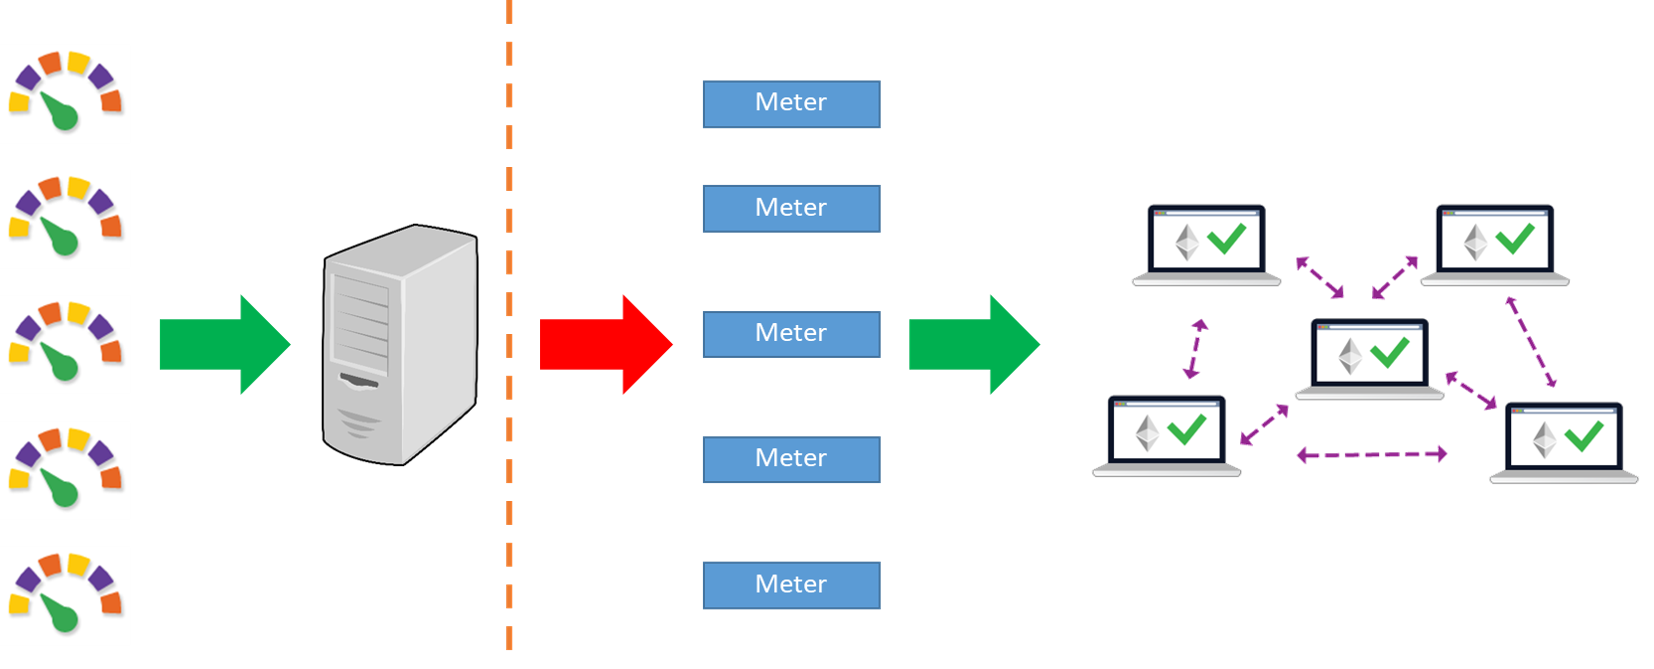
\includegraphics[width=\textwidth]{pull_push_monitoringserver}
    \caption{Meter Data gets pushed to the blockchain after getting pulled from the monitoring server}
    \label{fig:pull_push_monitoringserver}
\end{figure}
% must be able to keep track of the current reading and timestamp of the reading as well as the last reading and timestamp in order to calculate the difference of the two. It also has a unique identifier which is used to retrieve it in the smart contract.

\paragraph{Virtual Meters}

Smart meters get grouped in \textit{Virtual Meters}. The purpose of a Virtual Meter (VM) is to track the consumption of multiple Smart Meters across various rooms of a company building. As a result, the power consumption of each VM is a function of the power consumptions of its linked smart meters. % contributes to a room's consumption with a real coefficient, according to Equation \ref{roomcost}
\begin{figure}[htb]
    \centering
    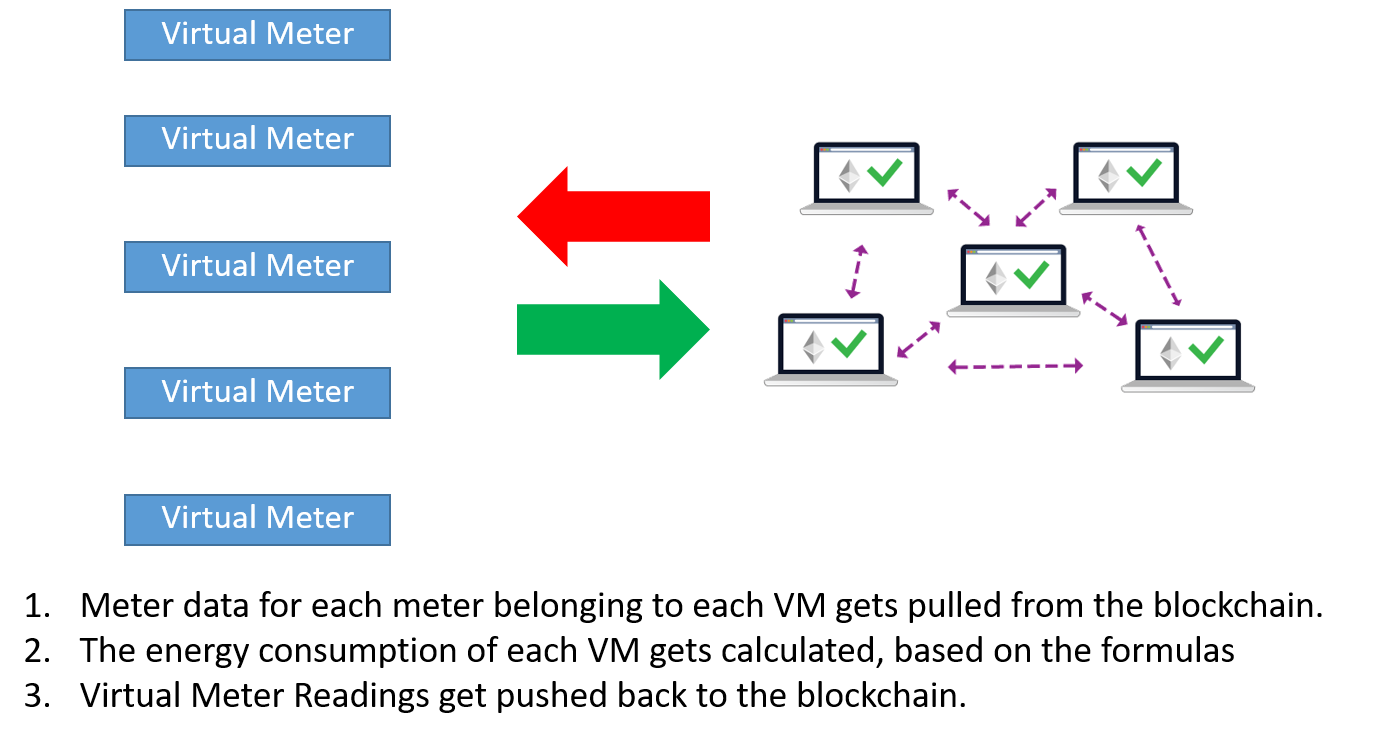
\includegraphics[width=\textwidth]{virtual_meters}
    \caption{The consumption of Virtual Meters gets calculated from the consumption of their associated Smart Meters.}
    \label{fig:virtual_meters_consumption}
\end{figure}

The formula that describes each Virtual Meter is supplied from an internal partner and is considered to be known. An example formula can be seen in Equation \ref{eq:formula}. $VM$ is a Virtual Meter, $ELT$ and $KMZ$ represent Smart Meters and $F$ are constants.

\begin{equation} \label{eq:formula}
    \begin{aligned}
        VM15= \\
        & (ELT46-(ELT31+ELT16+ELT17+ELT35+ELT36))*F57
        \\
        + & (ELT35+ELT36-ELT18)*F27*F66
        \\
        + & (KMZ6-KMZ5)*(ELT16+ELT17+ELT18+ELT19+ELT20)\\
        & /KMZ2*F27*F66 
    \end{aligned}
\end{equation}

Due to the amount of involved complexity, each Virtual Meter pulls the values for all of its associated Smart Meters, it applies its corresponding formula to the readings off-chain and pushes back the value to the smart contract.

\subsection{Accounting Logic} \label{billing}

\textit{Business Units} and \textit{Departments} are terms used to describe the hierarchy for the accounting business logic of the company. Business Units are used for external accounting, while departments and their subdepartments are used for internal monitoring. In implementation terms, a Business Unit is equivalent to a Department.

A Department is composed of Virtual Meters, other Departments and Delegates. Virtual Meters get grouped in Departments. A Department can include other subdepartments of a lower tier. Finally, a Department may forward its consumption to other Departments called Delegates. A department's consumption is the sum of energy consumed by its Virtual Meters, its Departments and its Delegates. 

\begin{figure}[ht!]
    \centering
    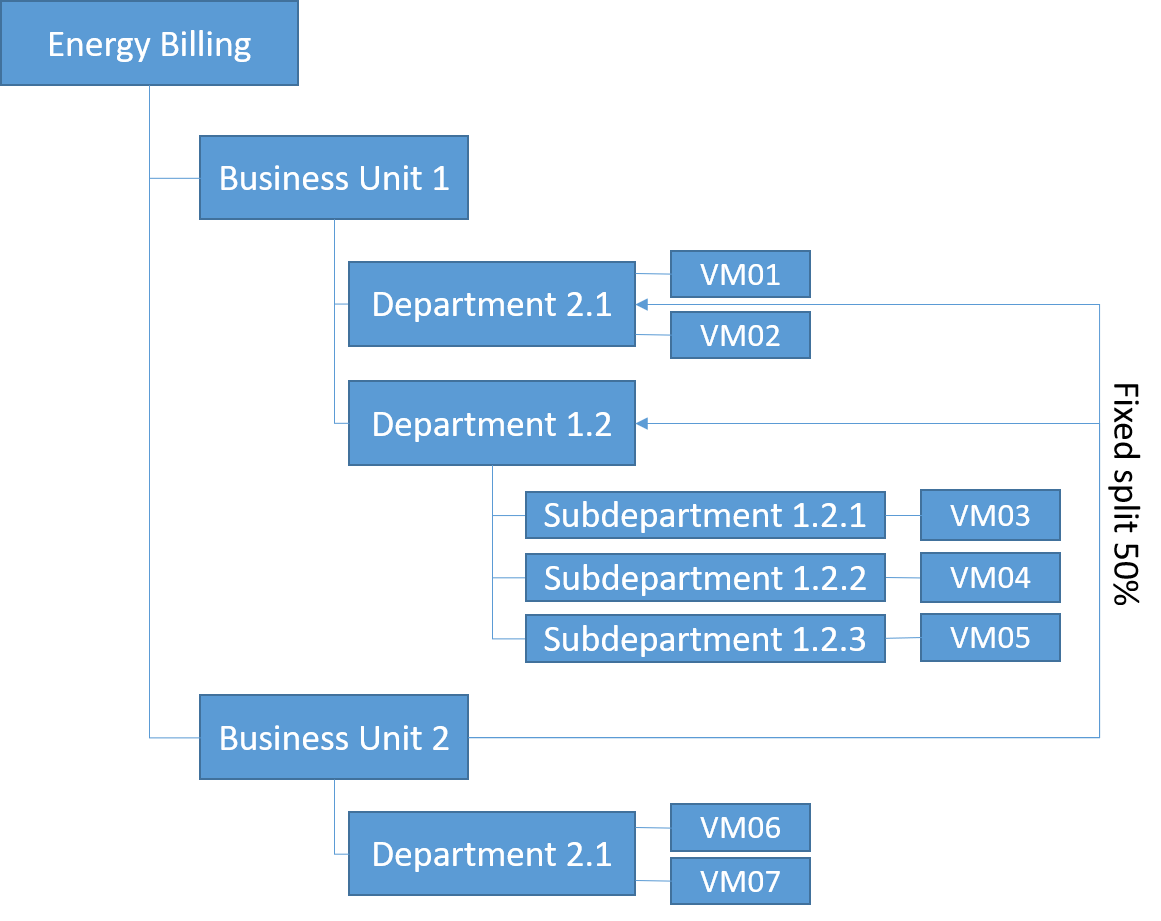
\includegraphics[width=.7\textwidth]{hierarchy}
    \caption{Relationship between Departments and Delegates.}
    \label{fig:hierarchy}
\end{figure}

Higher tier departments have the \texttt{headcount} property which defines the number of staff included in that Department. Delegation can be either through a headcount split or a fixed split. In headcount split, the amount that gets sent to each Delegate of the Department is proportional to their headcount percentage. Fixed split can only involve two Delegates, the first one receiving $X\%$ and the second one receiving $(100-X)\%$ of the Departments consumption, where $0<X<100$. As an example, in \ref{fig:hierarchy} Department 1.1 and 1.2 are fixed split delegates of Business Unit 2 and as a result their consumption is increased also by the consumption of Business Unit 2. After delegation, Business Unit 2 has its consumption cleared and will not be calculated towards the total Energy Billing.

\begin{figure}[H]
    \centering
    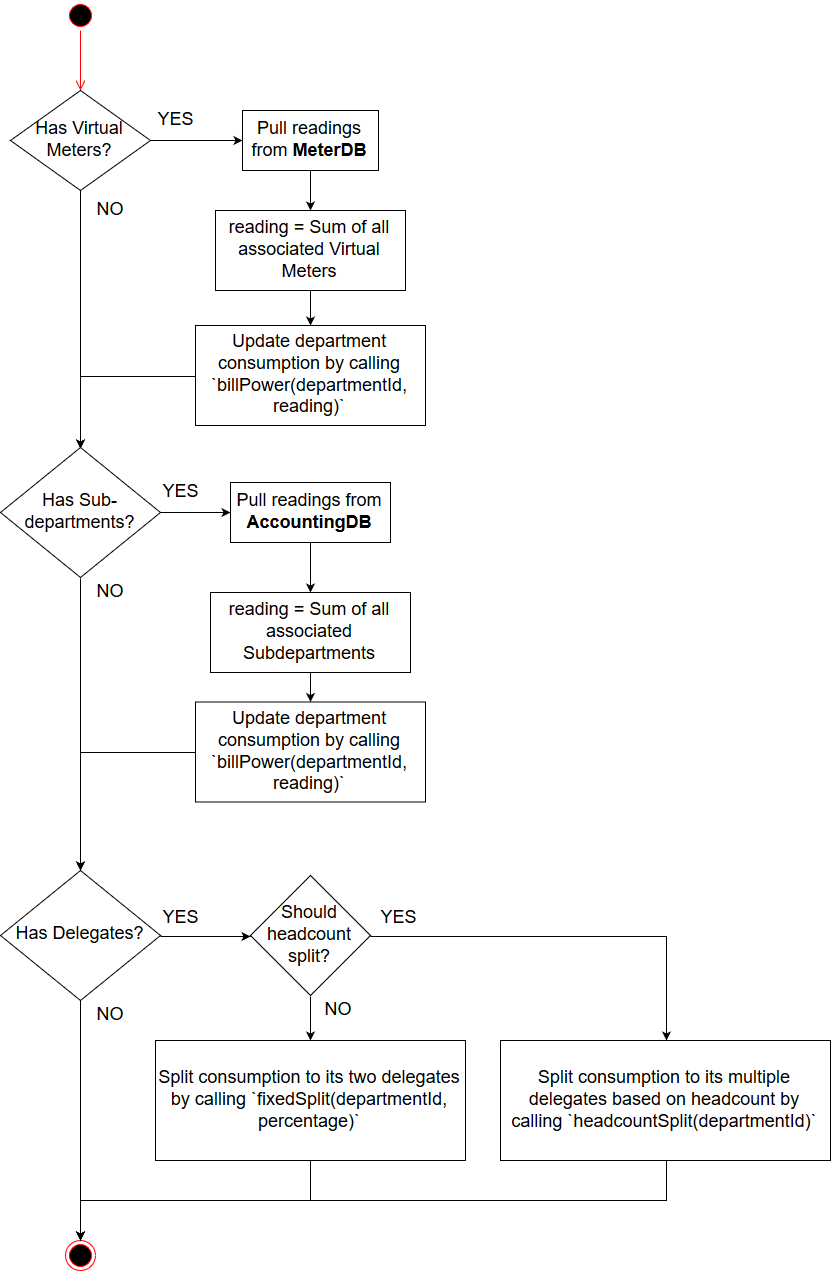
\includegraphics[width=\textwidth]{flowchart}
    \caption{Consumption calculation for a Department}
    \label{fig:consumption_flowchart}
\end{figure}

Due to the possibility of having multiple players of departments, in order to correctly calculate the final bill, the billing process starts from the inner-most tier of departments and iteratively moves outwards until the top-tier departments are reached.

\section{Smart Contracts} \label{ch:implementation:sc}
In this section we go over the implementation and the rationale of each developed smart contract. We explain the inner workings and provide tests of their functionality. % A thorough explanation how they interact with each other can be found in \ref{ch:results}.

\subsection{Access Control}
As discussed in Chapter \ref{ch:security} enforcing proper access control on critical functions of a smart contract is very important. It is common to find Access Control Lists (ACL) in enterprise environments which allow only selected participants to have to resources of various levels. This functionality does not exist by default in smart contracts. We proceed to describe the functionality of each of the mentioned roles for our smart contracts:
\begin{enumerate}
    \item Admin: Has full access to all contract functions
    \item Meter Manager: Can enable or disable a Meter at \texttt{MeterDB}.
    \item Meter: Can call the \texttt{ping} function of \texttt{MeterDB}
    \item Accountant: Can call the billing functions of \texttt{AccountingDB}
\end{enumerate}


% We utilize the base contract implementation of by DappSys \cite{dappsys} to create an access control list 

% The Aragon Project\footnote{Project aimed at creating DAOs} provides an ACL contract, however it was not used in the final version due to the complexity it introduced to our code\footnote{Aragon's contracts are architected towards creating fully upgradable DAOs, which would introduce considerable overheads and complexity to our code}. Instead, the DSAUTH pattern is used.

\subsection{Contract Registry}
Upgradable logic, call smart contract by name, versioning

\subsection{MeterDB}
MeterDB utilizes \ref{method3} to create a smart contract that keeps track of the last two consumed values and logged timestamps of a smart meter or a virtual meter. A meter must be approved by an entity who has been given access to the \texttt{activateMeter} through the ACL. 

EXPLAIN ASSUMPTIONS FOR DESIGN, NON ITERABLE BUT ITS OK. 

Each meter has its own ID. We use the pattern. Deleting a meter sets the active status to false. We iterate over the array of meters. There are software engineering patterns \cite{crud} that allow more proper usage, however they cost a lot more gas. 


\subsection{Cost - Profit Management}
We follow the same pattern as with meters for storing cost centers. We define 

\section{Client Side}

We utilize Python to interact with the smart contracts and push data to them. We implement multiple command line interfaces which can be used for abstracting the complexity to an operator. Due to design, it can be dockerized and run on multiple blabla.

\subsection{Monitoring Server and REST API}
Due to having dumb meters, we cannot get dirctly. There is a monitoring server which has all the data. A rest api allows us to pull data on demand. API explanation in appendix.k

Could be implemented without monitoring server if each meter was smarter. 
Explain monitoring server.

\subsection{web3.py interaction}
Explain how web3.py interacts with monitoring server and sends data to Smart Contracts

\subsection{Python Bindings and Clients for all functionalities}
Explain python implementation

using pool to launch multiple meter instances.



